\documentclass[letter]{beamer}
%removed: handout (ignores "animations")

\usepackage[utf8]{inputenc}
\usepackage{graphicx}

\usetheme{AnnArbor}
%\usetheme{CambridgeUS}
\usecolortheme{beaver}

\title[IIC2333] % (optional, only for long titles)
{00 - Caracterización de Sistemas Operativos}
\subtitle{IIC2333 - Sistemas Operativos y Redes}
\author[C.Ruz] % (optional, for multiple authors)
{Cristian Ruz -- {\tt cruz@ing.puc.cl} }
\institute[PUC] % (optional)
{
  Departamento de Ciencia de la Computación\\
  Pontificia Universidad Católica de Chile
}
\date[2/2015] % (optional)
{Semestre 2-2015}
\subject{Informatik}

\AtBeginSection[]
{
  \begin{frame}
    \frametitle{Contenidos}
    \tableofcontents[currentsection]
  \end{frame}
}

\begin{document}

%---------------------------------------------------------------------
\frame{\titlepage}

%---------------------------------------------------------------------
\begin{frame}
\frametitle{Contenidos}
%\tableofcontents[currentsection]
\tableofcontents
\end{frame}


%---------------------------------------------------------------------
\section{Estructura de un sistemas operativos}

\begin{frame}
  \frametitle{¿Qué hace un Sistema Operativo?}
  
\end{frame}


\begin{frame}
  \frametitle{El Sistema Operativo en un Sistema Computacional}
  \framesubtitle{{\em Software}}
  
  \begin{center}
    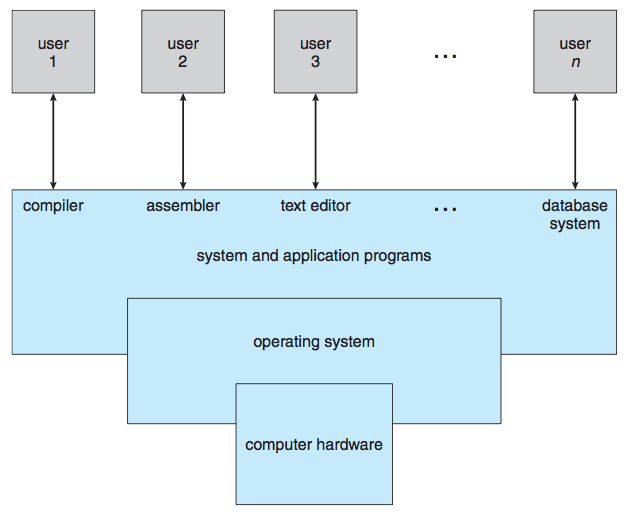
\includegraphics[width=9cm]{figs/00-ComponentesSistComp.png}
  \end{center}

  
\end{frame}

%---------------------------------------------------------------------
\begin{frame}
  \frametitle{¿Qué hace un Sistema Operativo?}

  No hace mucho por sí mismo (es como el gobierno)
  \begin{itemize}
    \item<2-> Y a la vez es fundamental
    \item<2-> Sería inútil sin programas/aplicaciones/usuarios (personas)
  \end{itemize}

  
\end{frame}

%---------------------------------------------------------------------
\begin{frame}
  \frametitle{¿Qué hace un Sistema Operativo?}

  Un Sistema Operativo tiene múltiples roles

  \begin{itemize}
    \item<2-> Para el usuario:
      \begin{itemize}
        \item<3-> Le permite {\bf utilizar los recursos} del computador
        \item<4-> Ejecutar programas, leer archivos, efectuar cálculos \ldots \onslide<5->{de manera fácil y rápida}
      \end{itemize}
    \item<6-> Para el sistema computacional:
      \begin{itemize}
        \item<7-> Un {\bf administrador de recursos} 
          \begin{itemize}
            \item<8-> Selecciona y provee los recursos necesarios
            \item<8-> Permite que se usen de manera eficiente
            \item<9-> ¿Qué es {\em eficiente} para: mainframe, virtual manager, sistema móvil?
          \end{itemize}
        \item<10-> Un {\bf programa de control} ... \onslide<11->{que evita el uso indebido}
          \begin{itemize}
            \item<12-> No ``botar'' otros programas en ejecución
            \item<12-> No sobreescribir por error el sistema operativo
            \item<12-> Evitar que un usuario se apropie del sistema
          \end{itemize}
      \end{itemize}
  \end{itemize}

\end{frame}


%---------------------------------------------------------------------
\begin{frame}
  \frametitle{¿Qué es un Sistema Operativo?}

  ¿Qué incluye?
  \begin{itemize}
    \item<2-> ¿Interfaz gráfica?
    \item<2-> ¿Editores?
    \item<2-> ¿Línea de comando?
  \end{itemize}
  
  \onslide<3->{¿De qué tamaño es? (¿Megas? ¿Kilos? ¿Gigas?)}\footnote{http://www.informationisbeautiful.net/visualizations/million-lines-of-code/}
  \begin{itemize}
    \item<4-> Windows 7: $\sim 40\times 10^6$ líneas de código
    \item<4-> Linux: $\sim 15 \times 10^6$ líneas de código
  \end{itemize}

  \onslide<4->{Entonces, el S.O. es ``lo que hay'' disponible}
  \begin{itemize}
    \item<4-> Lo que obtenemos de Microsoft/Apple
    \item<4-> Lo que bajamos de Linux
  \end{itemize}
\end{frame}

%---------------------------------------------------------------------
\begin{frame}
  \frametitle{¿Qué es un Sistema Operativo?}

  Lo comúnmente aceptado:
  \begin{alertblock}<2->{Sistema Operativo}
  Sistema Operativo = Kernel + Programas del sistema
  \end{alertblock}
  
  \begin{block}<3->{Kernel}
  Un programa que {\bf siempre} se está ejecutando.
  Provee funcionalidad mínima: acceso a CPU, memoria, dispositivos.
  \end{block}
  
  \begin{block}<4->{Programas del sistema}
  Extienden las funciones del kernel.
  \end{block}


\end{frame}


%---------------------------------------------------------------------
\begin{frame}
  \frametitle{¿Sobre qué {\em hardware}?}
  
  Distintas arquitecturas
  \begin{itemize}
    \item<2-> Single-core
      \begin{itemize}
        \item Un procesador de propósito general
        \item Algunas funciones delegadas a procesadores especializados
      \end{itemize}
    \item<3-> Multi-core
      \begin{itemize}
        \item Mayor rendimiento: ¿$N$?
        \item Economía de escala
        \item Mayor confiabilidad (reliability)
      \end{itemize}
    \item<4-> Arquitectura en {\em cluster}
      \begin{itemize}
        \item Múltiples procesadores conectados por red 
        \item Mayor potencia de cómputo (HPC)
        \item Es necesario manejar balance de carga y consistencia de datos
      \end{itemize}
  \end{itemize}
  
  \begin{block}<5->{}
  Sistema operativo debe ser capaz de explotar las características de cada arquitectura
  \end{block}
\end{frame}
%---------------------------------------------------------------------
\begin{frame}
  \frametitle{¿Por qué estudiar Sistemas Operativos?}
  \framesubtitle{(ó ¿por qué no?)}

  \begin{itemize}
    \item Piezas de software complejas
      \begin{itemize}
        \item Años de estudio y evolución
        \item ¿Cuántos sistemas operativos distintos manejan?
        \item ¿Cuántos sistemas operativos distintos usarán?
      \end{itemize}
    \item Un Sistema Operativo tiene múltiples desafíos:
      \begin{itemize}
        \item ¿Cómo proveer sistemas de alto rendimiento?
        \item ¿Cómo consumir la menor cantidad de energía?
        \item ¿Cómo asegurar que un usuario no altere datos o programas privados?
      \end{itemize}
  \end{itemize}

\end{frame}


%---------------------------------------------------------------------
\section{Evolución de Sistemas Operativos}


\begin{frame}
  \frametitle{Versión 1.0}

  Objetivo: acceder transparentemente a {\em hardware}
  \begin{itemize}
  \item<2-> ¿Cómo?: API para acceder a instrucción de {\em hardware} y conjunto de {\em drivers}
        para dispositivos.
  \item<3-> Supuestos:
    \begin{itemize}
      \item Sólo un usuario accede simultáneamente al computador
      \item Ningún usuario/programa hace uso malicioso del {\em hardware}
    \end{itemize}
  \item<4-> Problemas:
    \begin{itemize}
      \item Baja utilización de {\em hardware}: CPU inutilizada mientras se accede a disco
      \item Usuario debe esperar que un programa termine antes de utilizar otro
    \end{itemize}
  \end{itemize}
\end{frame}
%---------------------------------------------------------------------
\begin{frame}
  \frametitle{Versión 2.0}

  Objetivo: ejecutar múltiples programas simultáneamente. {\bf Multiprogramación}
  \begin{itemize}
  \item<2-> ¿Cómo?: Si un proceso se bloquea, ejecutar otro.
  \item<3-> Supuestos:
    \begin{itemize}
      \item Ningún programa utilizará la CPU demasiado tiempo (programas cooperativos)
      \item Ningún programa sobreescribirá datos de otro programa
    \end{itemize}
  \item<4-> Métodos:
    \begin{itemize}
      \item {\em Preemption}: capacidad de {\em expropiar} la CPU a un programa
      \item {\em Protección de memoria}: definir secciones de memoria para cada programa
    \end{itemize}
  \end{itemize}
\end{frame}

%---------------------------------------------------------------------
\begin{frame}
  \frametitle{Versión 3.0}

  Objetivo: que más de un usuario pueda utilizar simultáneamente el computador
  \begin{itemize}
  \item<2-> ¿Cómo?: Dándole un tiempo a cada usuario ({\em multitasking})
  \item<3-> Problemas:
    \begin{itemize}
      \item Cada usuario quiere el mayor tiempo posible: {\em planificación y políticas de uso}
      \item Cada usuario quiere usar la mayor cantidad de memoria disponible: {\em virtualización de memoria}
      \item ¿Hasta cuántos usuarios/programas aceptar? ({\em thrashing})
    \end{itemize}
  \item<4-> Método: niveles de privilegio
    \begin{itemize}
      \item Programas de usuario (aplicaciones) son {\em no privilegiados}
      \item Programas de {\em kernel} son {\em privilegiados}
      \item Solo programas de {\em kernel} pueden modificar el sistema
    \end{itemize}
  \end{itemize}
\end{frame}



%---------------------------------------------------------------------

%\begin{frame}
%  \frametitle{¿Qué se le pide a un Sistema Operativo?}
%%explicarlos de manera natural
%
%  \begin{itemize}
%    \item<2-> Capacidad de ejecutar {\bf procesos} definidos por el usuario
%    \item<3-> Capacidad de {\bf multiprogramación}
%      \begin{itemize}
%        \item<4-> Múltiples procesos en memoria (¿y si no caben?)
%        \item<5-> Mover algunos a disco (¿cuáles?)
%        \item<5-> Mantener siempre uno en ejecución (¿cuál?)
%        \item<6-> Debe hacer planificación: {\bf job+CPU scheduling}
%        %\item Ejemplo vida real
%      \end{itemize}
%    \item<7-> Capacidad de {\bf time-sharing} o {\bf multitasking}
%      \begin{itemize}
%        \item<8-> Cambio frecuentes entre programas
%        \item<9-> Permite que múltiples usuarios utilicen el sistema
%        \item<9-> Permite aplicaciones interactivas
%      \end{itemize}
%    \item<10-> Capacidad de administrar la {\bf memoria} del sistema
%      \begin{itemize}
%        \item<11-> Cada proceso requiere memoria, pero ésta es limitada
%        \item<12-> Swapping ... \onslide<13-> memoria virtual
%      \end{itemize}
%    \item<14-> Capacidad de utilizar {\bf almacenamiento no-volátil}
%  \end{itemize}
%\end{frame}

%---------------------------------------------------------------------
\begin{frame}
  \frametitle{¿Cómo funciona el Sistema Operativo?}
%explicarlos de manera natural
  
  \begin{block}{Si está siempre ejecutando, ¿cuándo le toca al usuario?}
    \onslide<2->{Los Sistemas Operativos son manejados por {\em interrupciones}/{\em trap}s.}
  \end{block}
  
  \onslide<3->{Mientras nadie (usuario/programa) lo llame, el S.O. no hace nada.}
  \begin{itemize}
    \item<4-> {\em Trap}: interrupción generada por software
      \begin{itemize}
        \item Error o solicitud de un programa
        \item Por cada solicitud, el S.O. toma una acción
      \end{itemize}
    \item<5-> S.O. debe asegurar que errores en un programa no afecten a otro
      \begin{itemize}
        \item<6-> ¿Qué pasa si un programa entra en un loop infinito?
        \item<6-> ¿Si un programa trata de modificar memoria de otro programa? ¿o del S.O.?
        \item<7-> Habría que asegurar que solo un proceso puede estar en modo ejecutable
      \end{itemize}
    \item<8-> Pero el S.O. sí debería poder modificar la memoria de otro programa, para cargarlo/descargarlo  
  \end{itemize}

\end{frame}

%---------------------------------------------------------------------
\begin{frame}
  \frametitle{Modos de operación de un Sistema Operativo}

  \begin{center}
    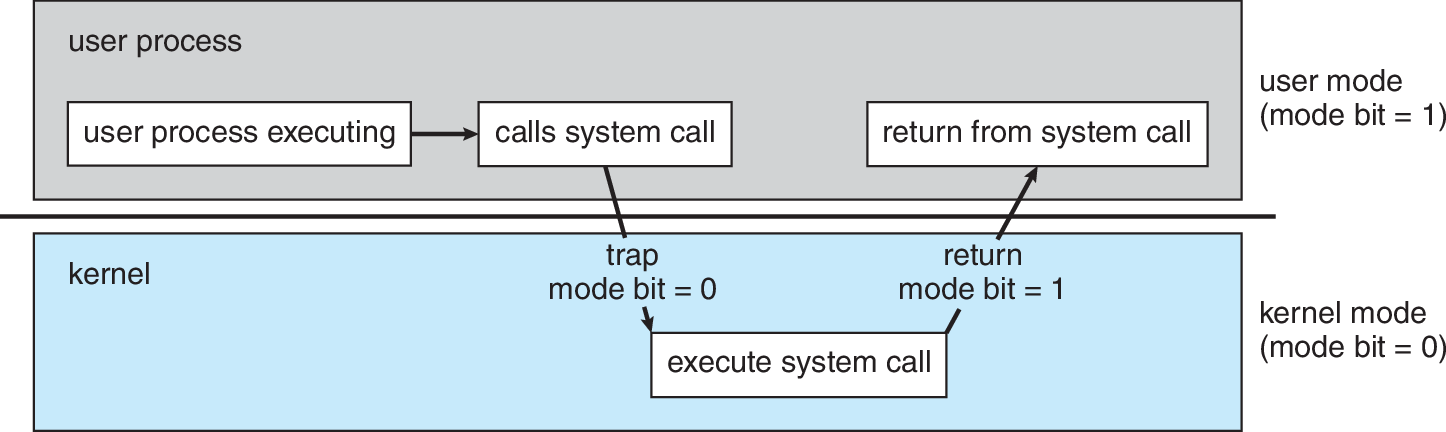
\includegraphics[width=8cm]{figs/00-1_10.pdf}
  \end{center}
  
  Modo dual suportado por hardware: mode bit (0=kernel/1=user)
  
  \onslide<2->{{\bf Solo puede ser modificado por el S.O.} (¿por qué?)}

  \onslide<3->{Kernel mode, a.k.a. (Privileged $|$ Supervised $|$ Monitor $|$ System) mode}
  
  \begin{alertblock}<4->{Instrucciones privilegiadas}
    Solo pueden ejecutar en modo kernel
      \begin{itemize}
        \item Si se intenta ejecutar en mode=1, el hardware no la ejecuta y genera
              una interrupción para el S.O. 
              Evita acceso indebido de otros usuarios  

      \end{itemize}
  \end{alertblock}  
  \onslide<5->{Ej: cambio mode bit, llamada I/O, manejo timer, manejo de interrupciones}
  
\end{frame}
%---------------------------------------------------------------------
\begin{frame}
  \frametitle{Modos de operación de un Sistema Operativo}
  \framesubtitle{Multi-modos}
  
  Más de dos modos de operación, ¿para qué?
  
  \begin{itemize}
    \item<2-> Útil para virtualización
    \item<3-> VMM ({\em Virtual Machine Manager}) opera en modo intermedio
      \begin{itemize}
        \item Menos privilegios que S.O.
        \item Más privilegios que cada {\em Virtual Machine}
      \end{itemize}
  \end{itemize}

  \begin{center}
    \includegraphics<3->[width=6cm]{figs/00-1_20.pdf}
  \end{center}
\end{frame}

%---------------------------------------------------------------------
\begin{frame}
  \frametitle{Modos de operación de un Sistema Operativo}

  Programas de usuario hacen llamadas al sistema operativo
  para que ejecute acciones a nombre de ellos
  
  \begin{itemize}
    \item {\em syscall}, {\em trap}
  \end{itemize}
  
  \onslide<2->{¿Qué puede pasar si no hay bit mode? (Intel 8088 no lo tenía)}
  %caso de 8088 y MS-DOS. Un proceso en MS-DOS podía echarse el SO
  
  \begin{itemize}
    \item<3-> Mode bit permite protección de hardware
    \item<4-> Si un programa comete un acceso indebido o error, trap al S.O.
      \begin{itemize}
        \item S.O. termina el programa {\em abnormally}
      \end{itemize}
    \item<5-> ¿Cómo evitar que un programa no devuelva el control al SO?
      \begin{itemize}
        \item<6-> S.O. usa un timer que genera un trap a intervalo definido
        \item<6-> Timer también debe ser establecido en modo Kernel
      \end{itemize}
  \end{itemize}

\end{frame}

%---------------------------------------------------------------------
\begin{frame}
  \frametitle{Entonces \ldots}

  3 tareas fundamentales para un Sistema Operativo:
  
  \begin{itemize}
    \item Administración de procesos
    \item Administración de memoria
    \item Administración de dispositivos de E/S
  \end{itemize}
\end{frame}

%---------------------------------------------------------------------
%\begin{frame}
%  \frametitle{Tarea: Administración de Procesos}
%
%  Administración de la unidad principal de trabajo: {\bf proceso}.
%  
%  \onslide<2->{Un proceso necesita diversos recursos:}
%  \begin{itemize}
%    \item<3-> CPU, memoria, archivos, dispositivos IO
%    \item<3-> Más que un programa (programa es pasivo, proceso es activo)
%  \end{itemize}
%  
%  \onslide<4->{Hay procesos de usuario y procesos de sistema}
%  
%  \begin{block}<5->{{\bf SO es responsable de:}}
%  \begin{itemize}
%    \item<5-> Planificar procesos y threads en la CPU
%    \item<5-> Crear y borrar procesos de usuario y de sistema
%    \item<5-> Suspender y continuar procesos
%    \item<5-> Proveer mecanismos de sincronización
%    \item<5-> Proveer mecanismos de comunicación
%  \end{itemize}
%  \end{block}
%  
%\end{frame}

%---------------------------------------------------------------------
%\begin{frame}
%  \frametitle{Tarea: Administración de Memoria}
%
%  La interacción de la CPU es principalmente con la memoria.
%  
%  {\bf Memoria:}\onslide<2->{ Un arreglo contínuo de bytes, cada uno con su propia dirección.}
%  
%  \begin{itemize}
%    \item<3-> Instruction-fetch y data-fetch ocurren con la memoria
%    \item<3-> Aún las lecturas de disco o de IO deben pasar por memoria
%    \item<4-> Las direcciones de un programa deben ser mapeadas a direcciones absolutas
%    \item<4-> Un uso eficiente requiere que haya múltiples procesos con su memoria listos para ejecutar
%  \end{itemize}
%  
%  \begin{block}<5->{{\bf SO es responsable de:}}
%  \begin{itemize}
%    \item<5-> Mantener un registro de los sectores de memoria utilizados y por quién
%    \item<5-> Determinar qué procesos o parte de ellos deben ser cargados y descargados
%    \item<5-> Asignar y deasignar espacios de memoria
%  \end{itemize}
%  \end{block}
%
%\end{frame}

%---------------------------------------------------------------------
%\begin{frame}
%  \frametitle{Tarea: Administración de Almacenamiento}
%  
%  \begin{center}
%    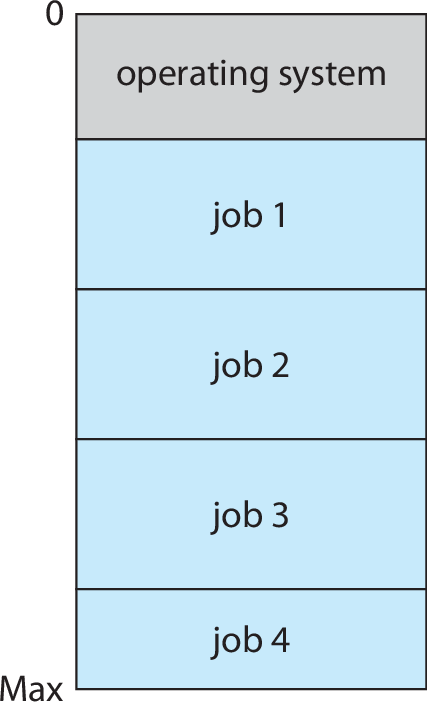
\includegraphics[width=3cm]{figs/00-1_09.pdf}
%  \end{center}
%
%  Distribución de memoria en un sistema de multiprogramación
%  
%\end{frame}

%---------------------------------------------------------------------
%\begin{frame}
%  \frametitle{Tarea: Administración de Almacenamiento}
%
%  Los sistemas de almacenamiento abstraen las propiedades físicas del medio
%  usando una unidad lógica de almacenamiento llamada \ldots \onslide<2->{{\bf archivo}}
%  
%  \onslide<2->{{\bf Archivo:}}\onslide<3->{ colección de datos relacionados, definida por su creador}
%  \onslide<4->{(sí, es algo muy general)}
%  
%  \onslide<5->{S.O. mapea archivos a ubicaciones dentro de medios físicos}
%  
%  \begin{itemize}
%    \item<5-> Distintos medios: discos magnéticos, ópticos, estado sólido, cintas
%    \item<5-> Distintas propiedades: velocidad de acceso, de transferencia, método de acceso (seq/aleatorio)
%    \item<5-> Debe definir quién puede acceder un archivo
%  \end{itemize}
%
%  \begin{block}<6->{{\bf SO es responsable de:}}
%  \begin{itemize}
%    \item<6-> Crear y borrar archivos, y directorios que permitan organizar archivos
%    \item<6-> Proveer primitivas para manipulación de archivos y directorios
%    \item<6-> Mapear archivos a almacenamiento secundario
%    \item<6-> Almacenar archivos en medios no-volátiles
%  \end{itemize}
%  \end{block}
%
%\end{frame}

%---------------------------------------------------------------------
%\begin{frame}
%  \frametitle{Tarea: Administración de Almacenamiento}
%
%  El almacenamiento secundario debe ser utilizado eficientemente
%  
%  \begin{itemize}
%    \item<2-> Su acceso suele limitar la velocidad de ejecución
%  \end{itemize}
%
%  \begin{block}<3->{{\bf SO es responsable de:}}
%  \begin{itemize}
%    \item Administrar espacio disponible
%    \item Asignación de destino de almacenamiento
%    \item Planificación de disco
%  \end{itemize}
%  \end{block}
%
%\end{frame}

%---------------------------------------------------------------------
%\begin{frame}
%  \frametitle{Caching}
%  \framesubtitle{El problema de la jerarquía de memoria}
%
%  Fundamental para asegurar un funcionamiento eficiente.
%  
%  Existe por la diferencia en los accesos a la jerarquía de memoria
%
%  \begin{center}
%    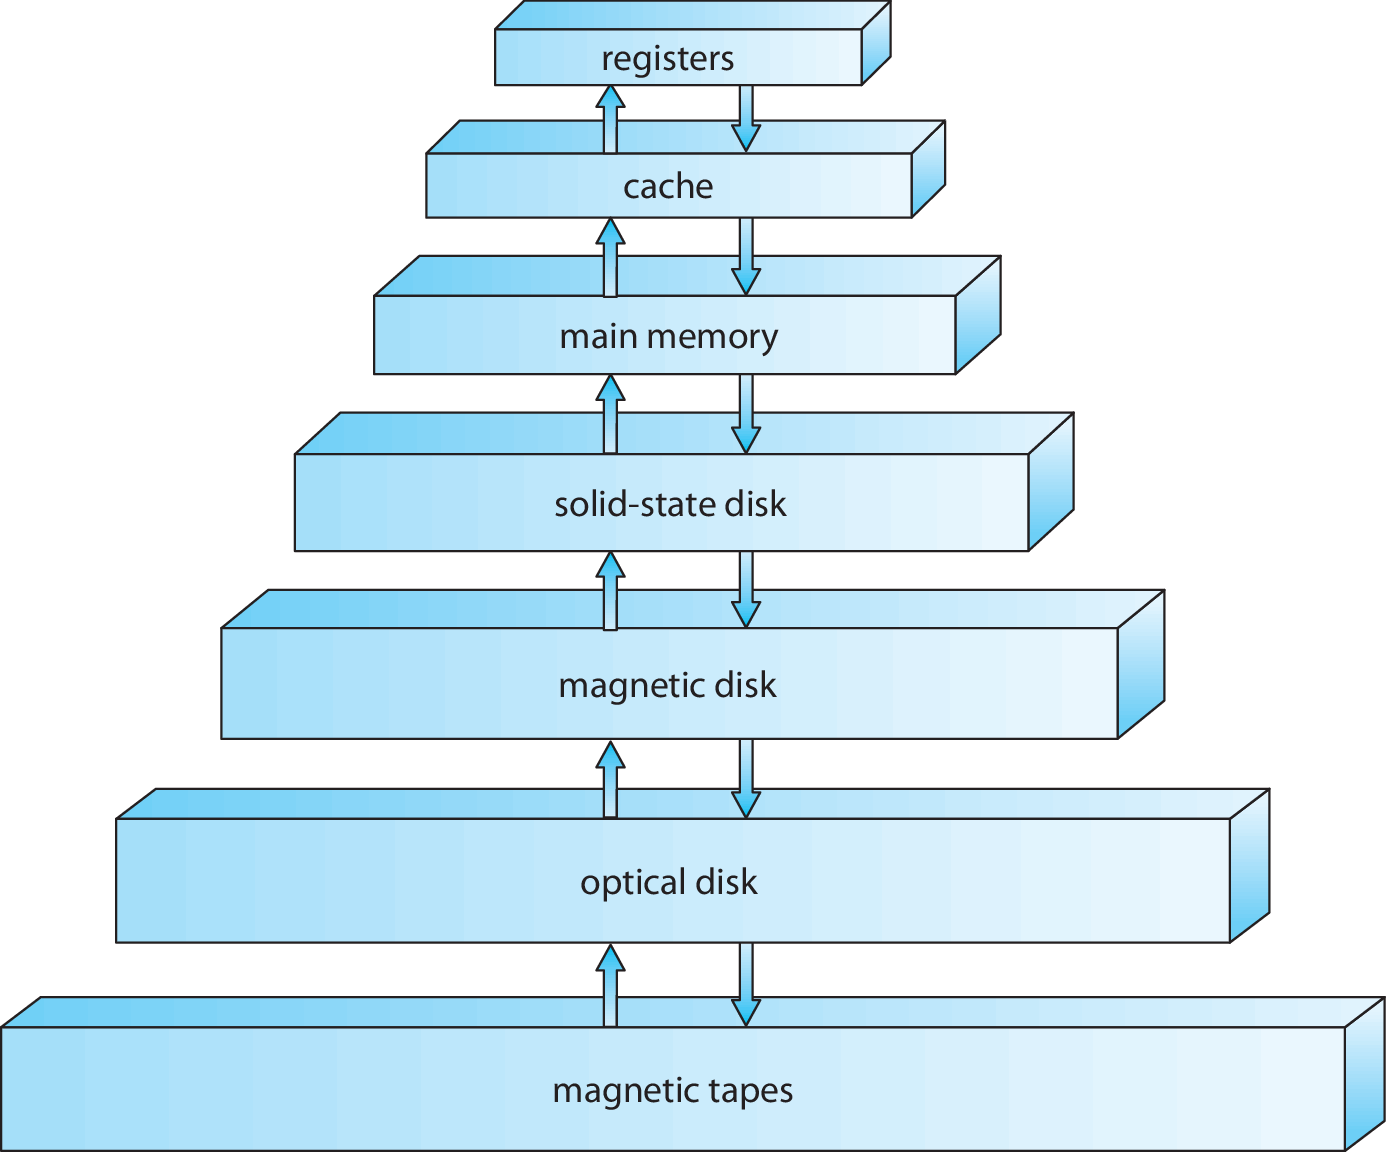
\includegraphics[width=6cm]{figs/00-1_04.pdf}
%  \end{center}
%
%\end{frame}

%---------------------------------------------------------------------

%---------------------------------------------------------------------
%\begin{frame}
%  \frametitle{Caching}
%  
%  \begin{itemize}
%    \item Datos viven en memoria principal
%    \item Al usarla se copia en almacenamiento más rápido
%    \item Al buscarla, se busca primero en caché
%    \item Si no se encuentra, se lee de memoria principal y se copia en caché
%  \end{itemize}
%  \onslide<2->{Caché}
%  \begin{itemize}
%    \item<2-> Registros: caché más cercano, administrado por programador/compilador
%    \item<2-> Cachés implementados en hardware, fuera del control de SO
%    \item<2-> Algunos datos deben ser borrados del caché, ¿cuáles?
%    \item<2-> Administración de caché es importante
%  \end{itemize}
%
%  \onslide<3->{¿Qué pasa cuando hay múltiples copias? ¿Con más de un proceso?}
%  
%  \onslide<4->{{\bf Coherencia de caché}} \onslide<5->{\ldots ¿Y en un ambiente distribuido?}
%  
%\end{frame}

%---------------------------------------------------------------------
%\begin{frame}
%  \frametitle{Caching}
%
%  Tiempos de acceso
%  
%  \begin{center}
%    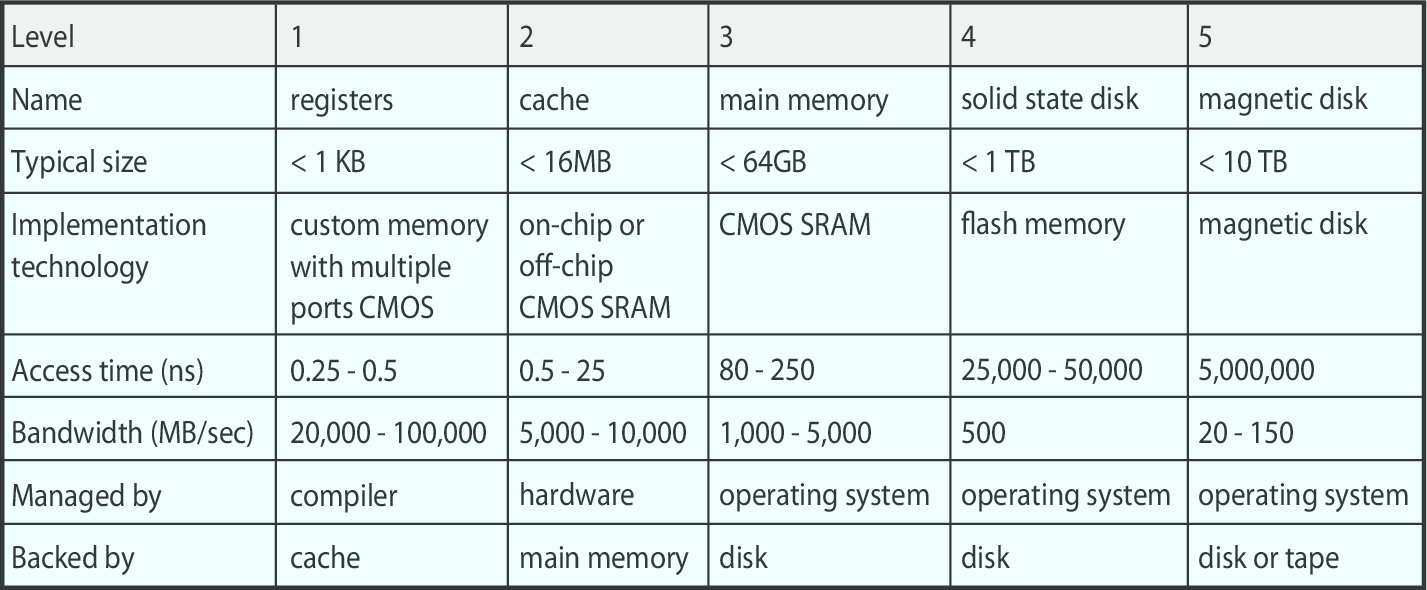
\includegraphics[width=10cm]{figs/00-1_11.pdf}
%  \end{center}
%
%\end{frame}

%---------------------------------------------------------------------
%\begin{frame}
%  \frametitle{Protección y Seguridad}
%
%  Ante múltiples usuarios, el acceso a datos debe ser regulado
%  
%  \onslide<2->{Hasta ahora \ldots}
%  \begin{itemize}
%    \item<3-> Hardware asegura que procesos solo pueden acceder memoria dentro de su espacio
%    \item<3-> Timer asegura que ningún proceso se quede sin devolver la CPU
%    \item<3-> Registros de control de dispositivos no son accesibles por usuarios
%  \end{itemize}
%
%  \onslide<4->{Sistemas de {\bf protección} controlan el acceso de procesos o usuarios a los recursos computacionales}
%  
%  \begin{itemize}
%    \item<5-> Un buen sistema de protección también puede sufrir de accesos indebidos
%  \end{itemize}
%
%  \onslide<6->{Un sistema de {\bf seguridad} debe defender de ataques externos e internos}
%  
%\end{frame}

%---------------------------------------------------------------------
%\begin{frame}
%  \frametitle{Protección y Seguridad}
%
%  Algunos requisitos de los sistemas de protección y seguridad
%  
%  \begin{itemize}
%    \item<2-> Distinción entre usuarios: nombre e identificador (userID, securityID)
%    \item<2-> Grupos de usuarios e identificadores de grupos
%    \item<2-> Asociación de privilegios/permisos 
%    \item<2-> Métodos seguros para escalar privilegios (setuid)
%  \end{itemize}
%  
%\end{frame}

%---------------------------------------------------------------------
%\section{Elementos y Servicios de un Sistema Operativo}
\section{Interfaces y Llamadas al sistema}

\begin{frame}
  \frametitle{Elementos y Servicios de un Sistema Operativo}

  At a glance \ldots
  
  \begin{center}
    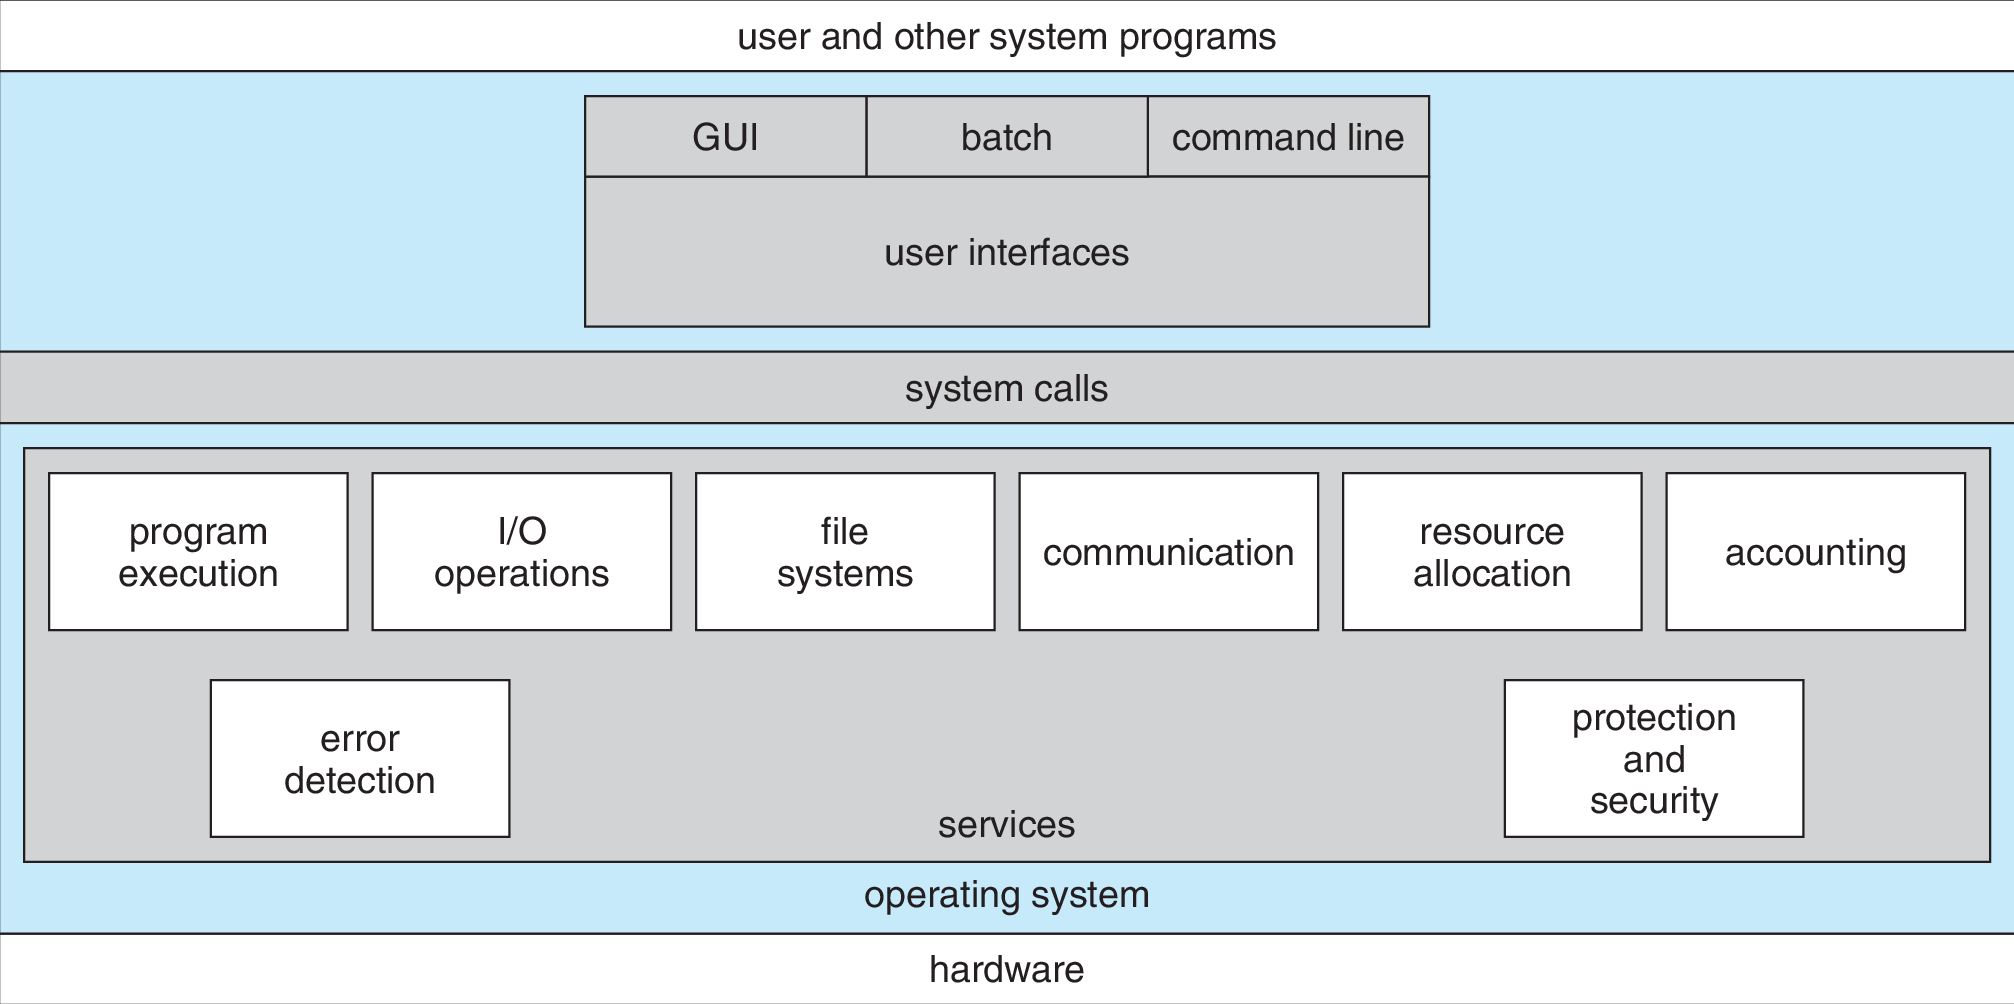
\includegraphics[width=11cm]{figs/00-2_01.pdf}
  \end{center}

\end{frame}

%---------------------------------------------------------------------
\begin{frame}
  \frametitle{Interfaces de Usuario (UI)}

  Varias alternativas \ldots
  \begin{description}
    \item[Command-Line Inteface (CLI)] Comandos se ingresan por teclado
    \item[Batch interface] Comandos se ingresan en archivos
    \item[Graphical User Interface (GUI)] Sistema de ventanas + {\em pointing-device}
  \end{description}
  

\end{frame}

%---------------------------------------------------------------------
\begin{frame}
  \frametitle{Interfaces de Usuario (UI)}
  \framesubtitle{Command-Line (línea de comandos)}
  
  También conocidos como {\bf shell}s
  
  \begin{itemize}
    \item<2->{\em Bourne shell}: Stephen Bourne, 1977, UNIX, {\tt /bin/sh}
    \item<2->{\em C shell}: Bill Joy, 1978, BSD UNIX, {\tt csh}
    \item<2->{\em TENEX C Shell}: Ken Greer, 1983, {\tt tcsh}
    \item<2->{\em Korn shell}: David Korn, 1983, {\tt ksh}
    \item<2->{\em Bourne-Again shell}: Brian Fox, 1989, {\tt bash}
    \item<2->{\em Z shell}: Paul Fastad, 1990, {\tt zsh}
  \end{itemize}
  
  \begin{itemize}
    \item<3->{\em MS-DOS prompt}: MS-DOS, Win95/98/Me, {\tt COMMAND.COM}
    \item<3->{\em Command Prompt}: {\tt cmd.exe} 
  \end{itemize}
\end{frame}
%---------------------------------------------------------------------
\begin{frame}
  \frametitle{Interfaces de Usuario (UI)}
  \framesubtitle{Command-Line (línea de comandos)}

  Uso común:
  \begin{itemize}
    \item Solicitar comando/instrucción al usuario y ejecutarlo
    \item Formato: {\tt prompt} {\tt comando} {\tt [parametros]} 
  \end{itemize}

  \onslide<2->{{\em Command Prompt} (símbolo del sistema)}
  \begin{itemize}
    \item<2->Indica que el sistema está lista para recibir un comando
    \item<2->Usualmente un texto terminado en {\tt \$}, {\tt \%}, {\tt \#}, {\tt :}, {\tt >}
  \end{itemize}

  \onslide<3->{Comandos simples:
  \begin{center}
     {\tt cruz\$ ls }
  \end{center}
  }

  \onslide<4->{Comandos con parámetros:
  \begin{center}
     {\tt jabaier@grima\# cp clase01.txt clase02.txt}
  \end{center}
  }
  
  \onslide<5->{Comandos con {\em wildcards}:
  \begin{center}
     {\tt jnavon@www[15:35]:> rm tareaSistOp.*}
  \end{center}
  }

\end{frame}

%---------------------------------------------------------------------
%\begin{frame}
%  \frametitle{Interfaces de Usuario (UI)}
%
%  \begin{center}
%    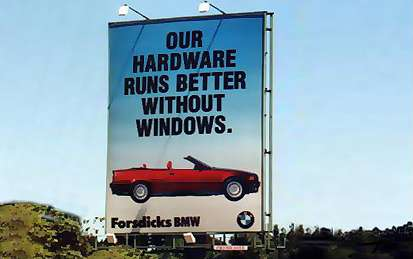
\includegraphics[width=10cm]{figs/00-noWindows.jpg}
%  \end{center}
%
%\end{frame}
%---------------------------------------------------------------------
\begin{frame}
  \frametitle{Interfaces de Usuario (UI)}
  \framesubtitle{Graphical User Interface (GUI)}

  Interfaz gráfica (para quienes no les gusta escribir comandos)
  
  \begin{itemize}
    \item<2-> Usualmente con un {\em pointing-device} y ventanas
    \item<2-> Métaforas: escritorio, íconos, carpetas, menúes
    \item<2-> Más allá de {\em pointing-device}: gestos y acciones visuales
  \end{itemize}
  
  \onslide<3->{Vienen de los $\sim$ 1970's}
  \begin{itemize}
    \item<4-> Investigación de Xerox Palo Alto Research Center (PARC)
    \item<4-> Primera interfaz gráfica: 1973
    \item<4-> Popularizados en 1980s: Apple Macintosh (Mac OS)
    \item<4-> Windows 1.0 agregó GUI a MS-DOS
  \end{itemize}


\end{frame}

%---------------------------------------------------------------------
\begin{frame}
  \frametitle{Interfaces de Usuario (UI)}
  \framesubtitle{Graphical User Interface (GUI)}

  Tradicionalmente UNIX/Linux han sido manejados por CLI,
  \onslide<2->{pero se han desarrollado muchas GUIs}
  \begin{itemize}
    \item<3-> CDE ({\em Common Desktop Environment}): Unix, OpenVMS
    \item<3-> X-Windows Systems: Xfce, KDE, GNOME (Unix/Linux)
  \end{itemize}
  
  \begin{center}
    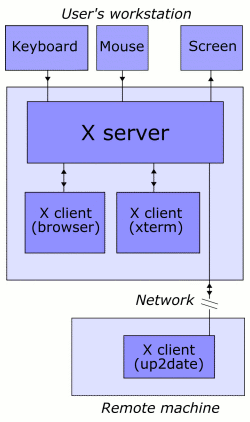
\includegraphics[width=3cm]{figs/00-Xwindows.png}
  \end{center}

\end{frame}

%---------------------------------------------------------------------
\begin{frame}
  \frametitle{Interfaces de Usuario (UI)}
  \framesubtitle{Graphical User Interface (GUI)}

  \begin{center}
    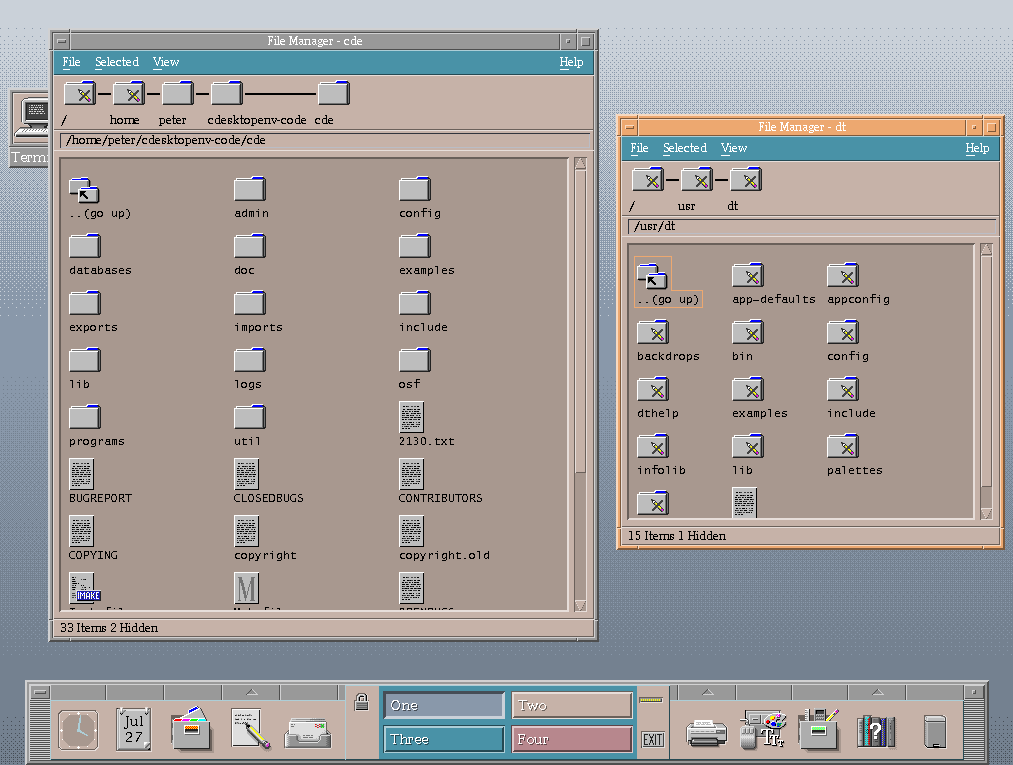
\includegraphics[width=8cm]{figs/00-CDE.png}
  
    CDE (Common Desktop Environment)
  \end{center}

\end{frame}

%---------------------------------------------------------------------
\begin{frame}
  \frametitle{Interfaces de Usuario (UI)}
  \framesubtitle{Graphical User Interface (GUI)}

  \begin{center}
    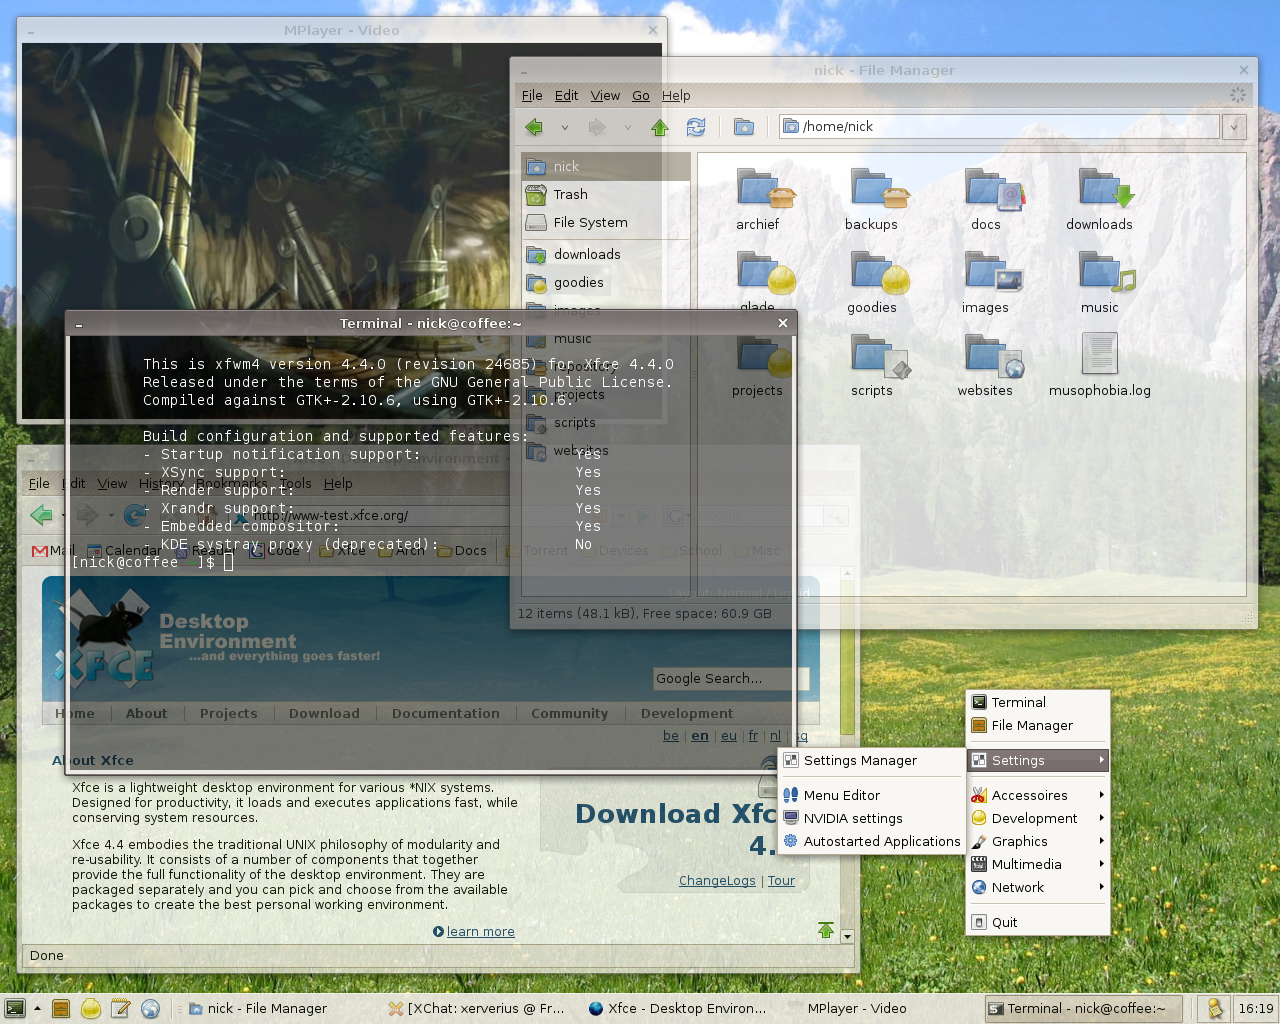
\includegraphics[width=8cm]{figs/00-XFCE.png}
  
    Xfce
  \end{center}

\end{frame}

%---------------------------------------------------------------------
\begin{frame}
  \frametitle{Interfaces de Usuario (UI)}
  \framesubtitle{Graphical User Interface (GUI)}

  \begin{center}
    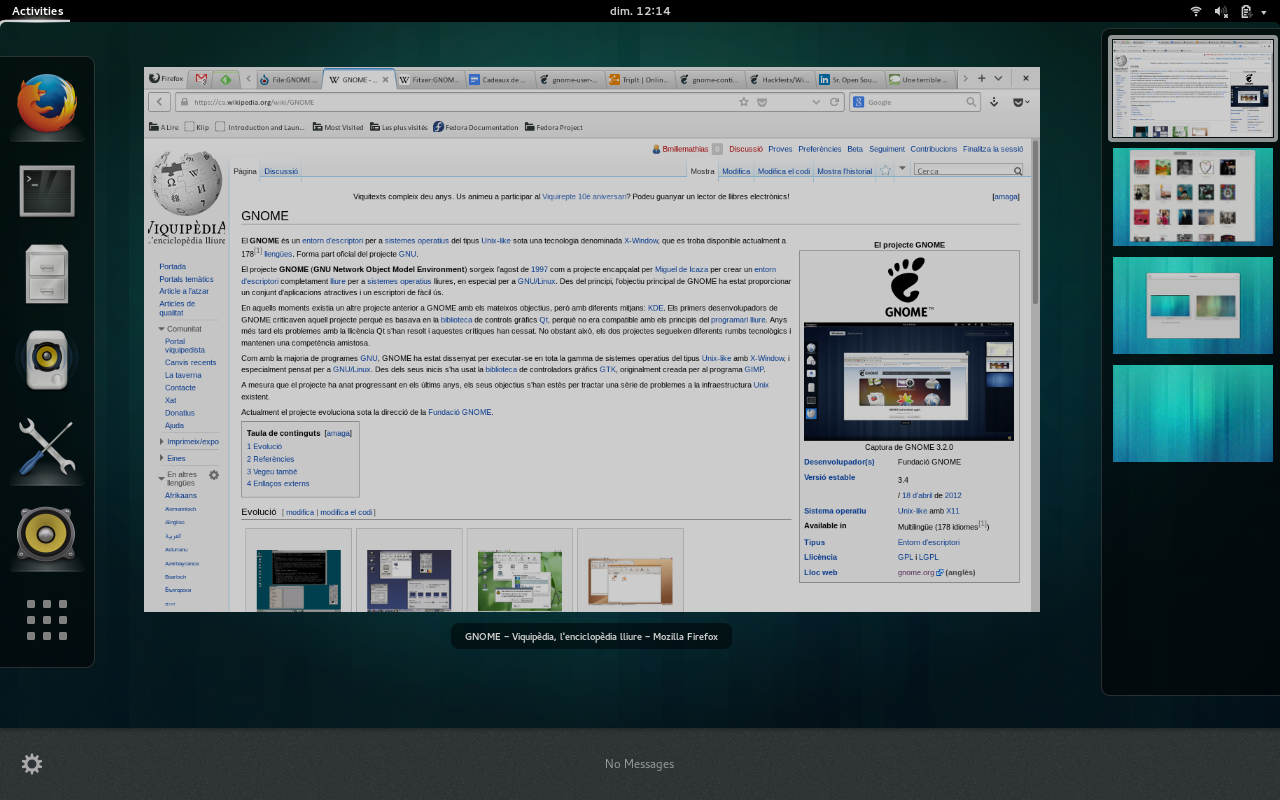
\includegraphics[width=10cm]{figs/00-GNOME.png}
  
    GNOME 
  \end{center}

\end{frame}

%---------------------------------------------------------------------
\begin{frame}
  \frametitle{Interfaces de Usuario (UI)}
  \framesubtitle{Graphical User Interface (GUI)}

  \begin{center}
    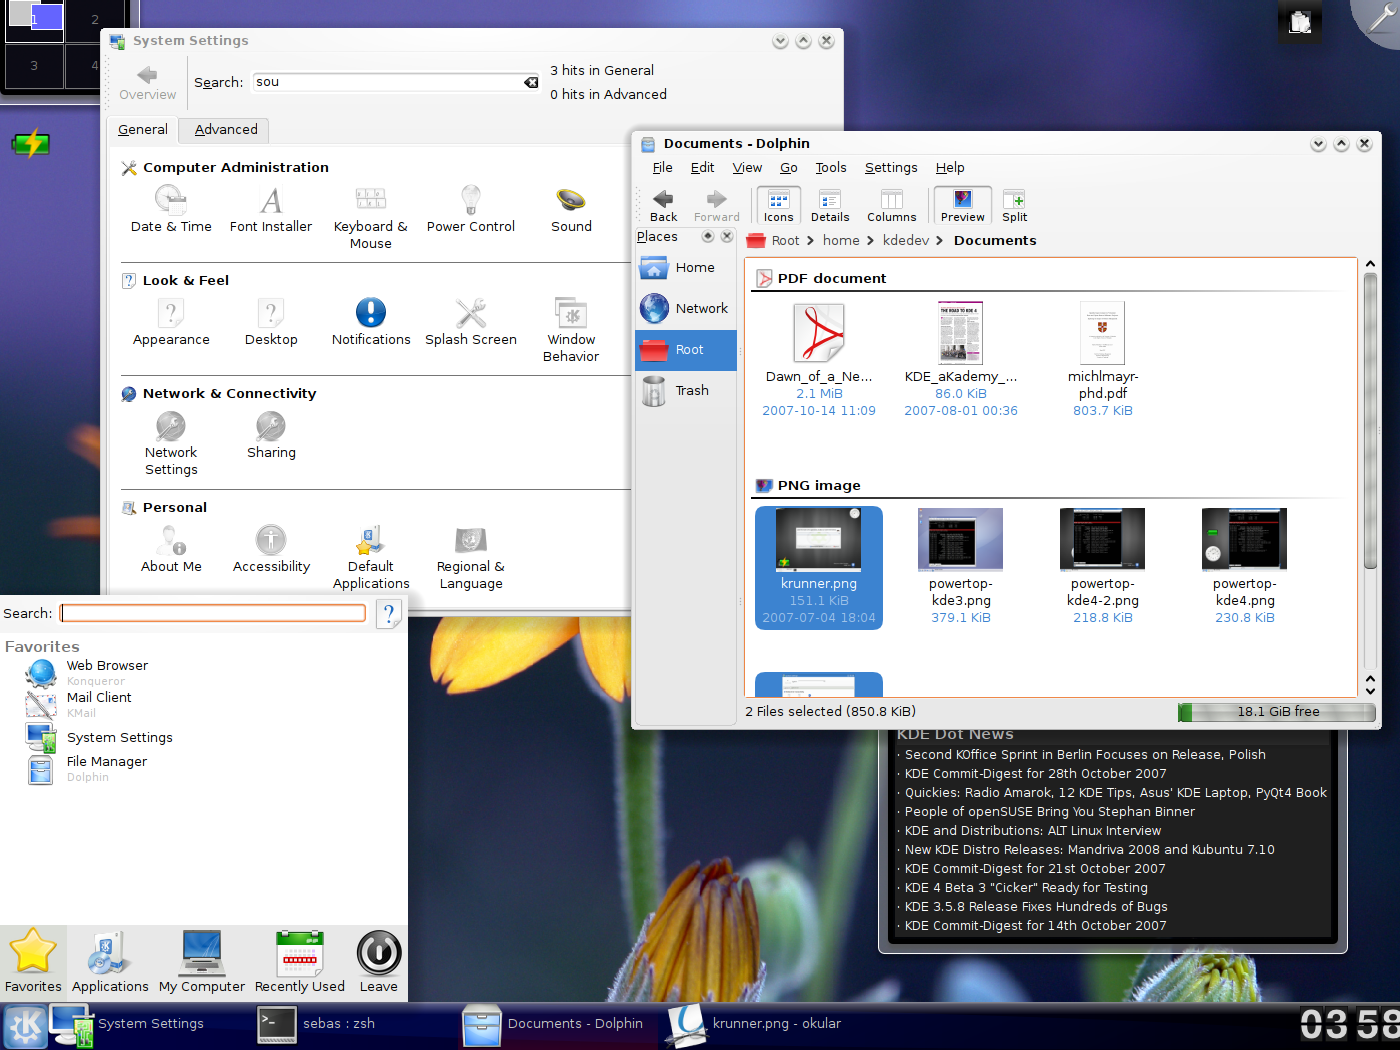
\includegraphics[width=8cm]{figs/00-KDE.png}
  
    KDE (K Desktop Environment)
  \end{center}

\end{frame}

%---------------------------------------------------------------------

\begin{frame}
  \frametitle{Llamadas al sistema}
  \framesubtitle{System Calls}
  
  Programas utilizan llamadas al sistemas frecuentemente
  
  \onslide<2->{Ej: {\tt copy source.txt dest.txt} ... ¿qué requiere?}
  \begin{itemize}
    \item<3-> Abrir {\tt source.txt}
      \begin{itemize}
        \item ¿Existe?
        \item ¿Tiene permisos?
      \end{itemize}
    \item<4-> Abrir {\tt dest.txt}
      \begin{itemize}
        \item ¿Existe? ¿se reemplaza?
        \item ¿Se puede escribir?
      \end{itemize}
    \item<5-> Lectura/escritura en disco requiere llamadas al sistema
    \item<6-> Terminar el programa en caso de error, requiere llamadas al sistema
  \end{itemize}
  \onslide<7->{\ldots pero el programador no quiere programar todas las llamadas}

\end{frame}

%---------------------------------------------------------------------
\begin{frame}
  \frametitle{Llamadas al sistema}
  \framesubtitle{API: Application Programming Interface}
  
  Sistemas Operativos proveen una API para el programador.
  \begin{itemize}
    \item<2-> Windows API
    \item<3-> POSIX API (UNIX, Linux, MacOS X), a través de {\tt libc}
    \item<4-> Java API (para la JVM)
  \end{itemize}

  \onslide<5->{¿Cómo usarla?}
  \onslide<6->{
  \begin{center}
    Ejemplo: {\tt man read}
  \end{center}  
  }
  
\end{frame}

%---------------------------------------------------------------------
\begin{frame}
  \frametitle{Llamadas al sistema}

  \begin{center}
    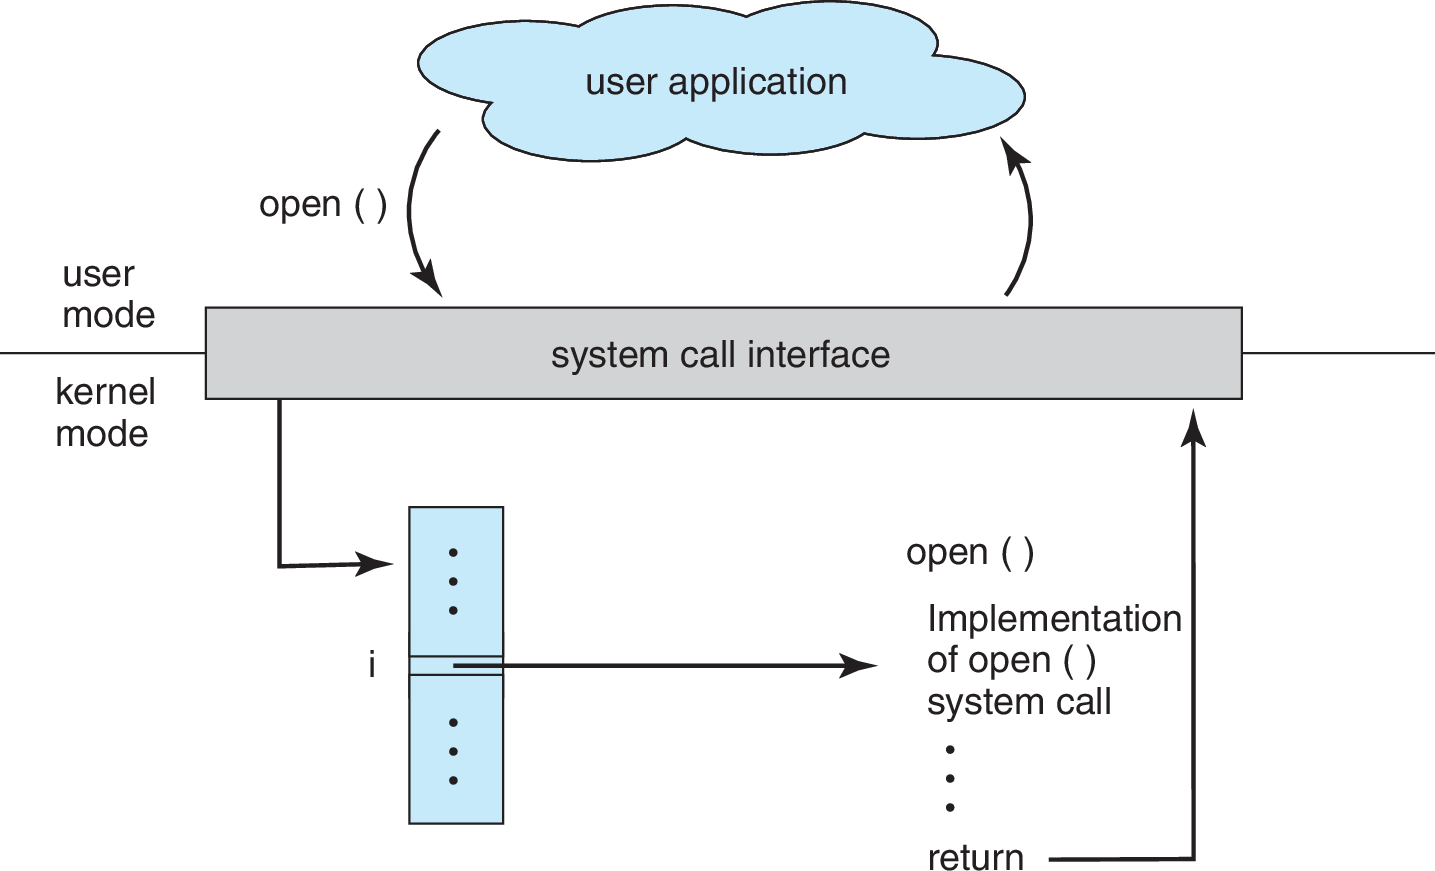
\includegraphics[width=11cm]{figs/00-2_06.pdf}
  \end{center}

\end{frame}

%---------------------------------------------------------------------
\begin{frame}
  \frametitle{Llamadas al sistema}

  \begin{center}
    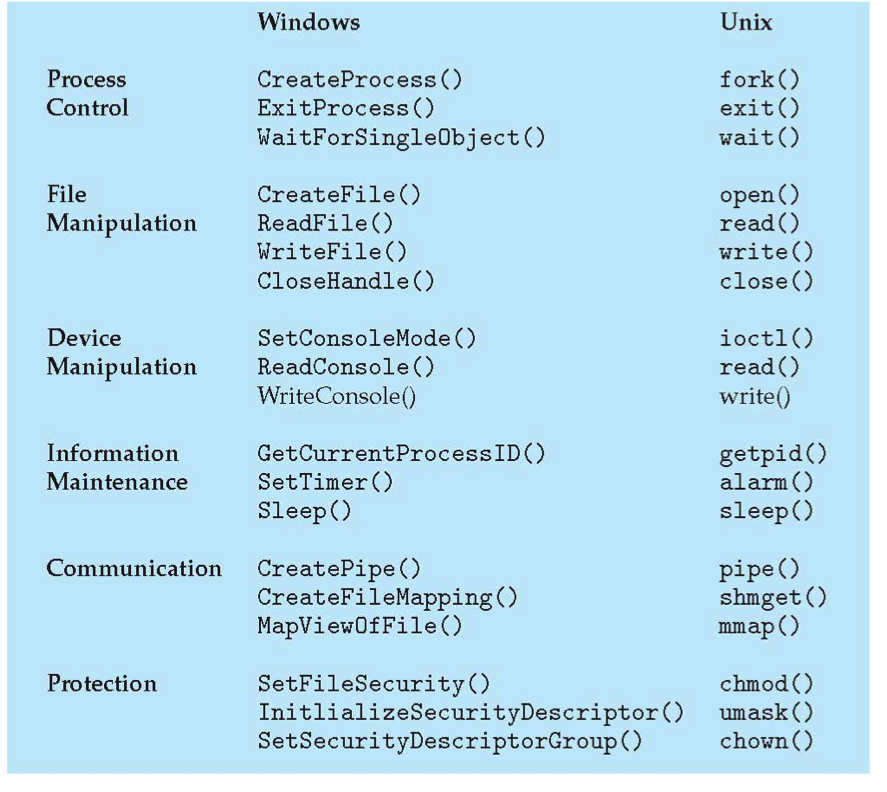
\includegraphics[width=8cm]{figs/00-syscalls.png}
  \end{center}

\end{frame}

%---------------------------------------------------------------------
%\section{Decisiones de diseño}

%\begin{frame}
%  \frametitle{Decisiones de diseño}
%  ¿Cuál es la mejor forma de diesñar un Sistema Operativo?
%  
%  \onslide<2->{(si se supiera no habrían {\em OS wars})}
%
%  \begin{itemize}
%    \item<3-> Uso de {\bf estructuras de datos} apropiadas
%    \item<4-> Aplicando principios de {\bf ingeniería de software}
%    \item<5-> Aprovechando las capacidades que permite la {\bf arquitectura del hardware}  
%  \end{itemize}
%
%\end{frame}

%---------------------------------------------------------------------
%\begin{frame}
%  \frametitle{Decisiones de diseño}
%
%%  \begin{itemize}
%%    \item {\bf Mecanismo}: {\em cómo} se implementa una funcionalidad (decisión estática)
%%      \begin{itemize}
%%        \item Ej: Mecanismo para asignar prioridades a procesos.
%%      \end{itemize}
%%    \item {\bf Política}: {\em qué} decisión se va a implementar
%%      \begin{itemize}
%%        \item Ej: Bajo qué criterio se asignan prioridades
%%      \end{itemize}
%%  \end{itemize}
%%  
%  \onslide<2->{
%  Principio de {\bf separación de preocupaciones} ({\em separation of concerns})
%  \begin{itemize}
%    \item {\em Microkernels} definen un conjunto pequeño de primitivas
%    \item Mecanismo deberían {\em de propósito general}
%  \end{itemize}
%  }
%  
%\end{frame}

%---------------------------------------------------------------------
%\begin{frame}
%  \frametitle{¿En qué lo programo?}
%
%  ¿En qué se programa un sistema operativo?
%  \begin{itemize}
%    \item<2-> Los primeros ... en {\em assembler}
%    \item<3-> Más modernos en C, C++ (Windows, Linux)
%    \item<4-> Actuales incluyen muchos lenguajes
%      \begin{itemize}
%        \item Bajo nivel en assembler
%        \item Interacciones principales en C
%        \item Utilidades de alto nivel en lenguaje interpretado (python, perl)
%      \end{itemize}
%  \end{itemize}
%  
%  \onslide<5->{Al usar un lenguaje de alto nivel es más fácil hacer un {\bf port}}
%  \begin{itemize}
%    \item <6-> MS-DOS fue escrito en Assembler de Intel 8088
%    \item <6-> Para otras arquitecturas se requiere un {\bf emulador}
%  \end{itemize}
  
%\end{frame}
%---------------------------------------------------------------------
\begin{frame}
  \frametitle{Estructura: MS-DOS}
  
  ¿Sistemas {\bf monolíticos} o sistemas {\bf modulares}?
  
  \onslide<2->{Algunos ni siquiera tienen estructura}
  \begin{itemize}
    \item<3-> MS-DOS: sistema monolítico simple
    \item<3-> Nadie pensó que sería tan popular
    \item<3-> Intel 8088 no tenía protección de {\em dual mode}
    \item<3-> ¿Problemas? \onslide<4->{Seguridad}
  \end{itemize}
  
  \begin{center}
    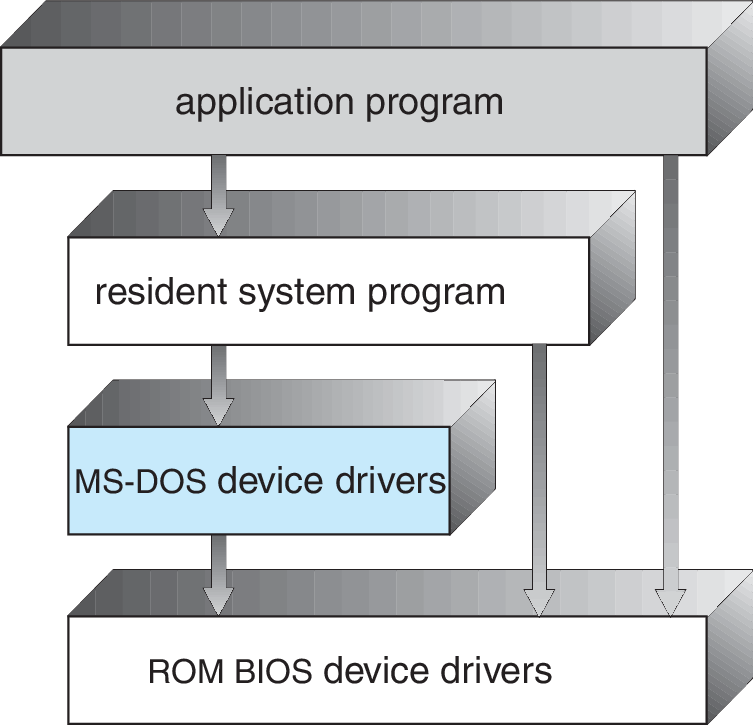
\includegraphics[width=4cm]{figs/00-2_11.pdf}
  \end{center}
  
  
\end{frame}

%---------------------------------------------------------------------
\begin{frame}
  \frametitle{Estructura: UNIX}

  UNIX: Estructura monolítica diseñada de acuerdo al {\em hardware}
  
  \begin{center}
    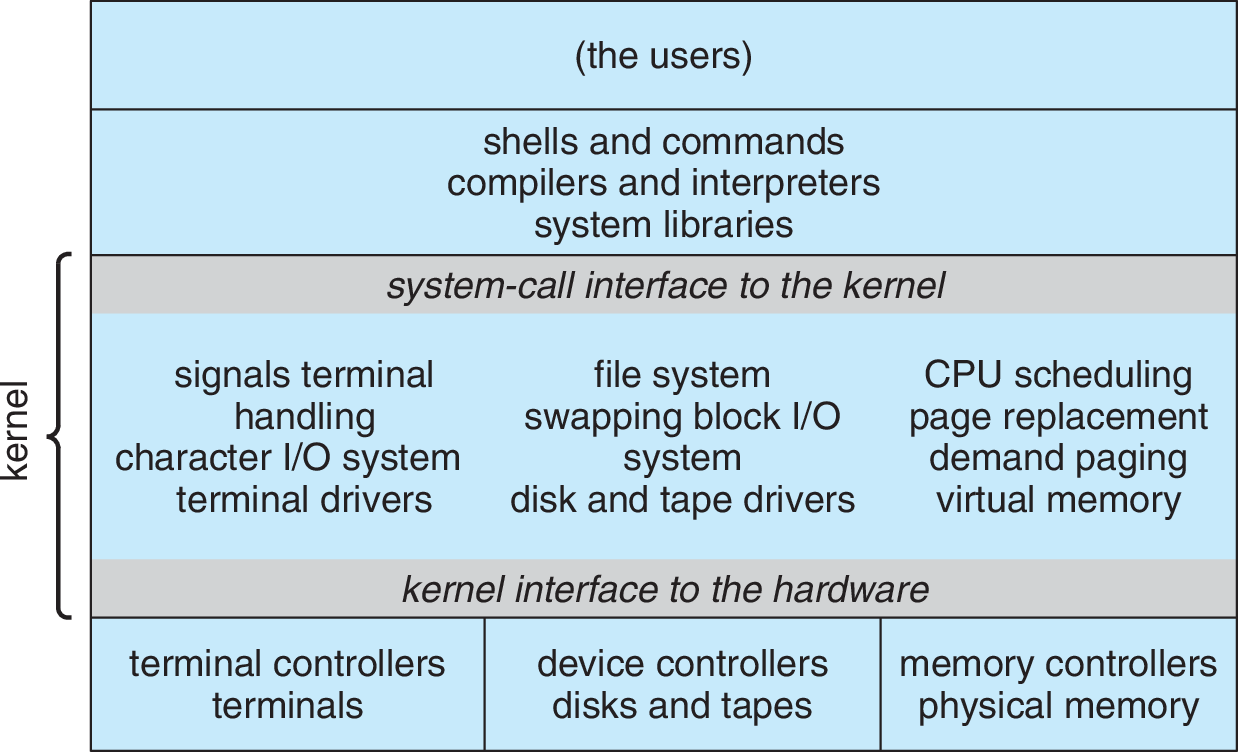
\includegraphics[width=8cm]{figs/00-2_12.pdf}
  \end{center}

  \onslide<2->¿Problemas? \onslide<3->{Dificultad de mantenimiento}
\end{frame}

%---------------------------------------------------------------------
\begin{frame}
  \frametitle{Estructura: diseño por capas}

  Capas se diseñan por niveles más {\em abstractos} de funcionalidad
  
  \begin{itemize}
    \item Capa $M$ invoca llamadas sobre capa $M-1$
    \item<2-> Ventaja: Facilidad de {\em debugging}
    \item<3-> Desventaja: dificultad de definición de capas (¿a qué nivel va qué funcionalidad?)
    \item<3-> Desventaja: eficiencia (¿cuántas capas?)
  \end{itemize}
  
  \begin{center}
    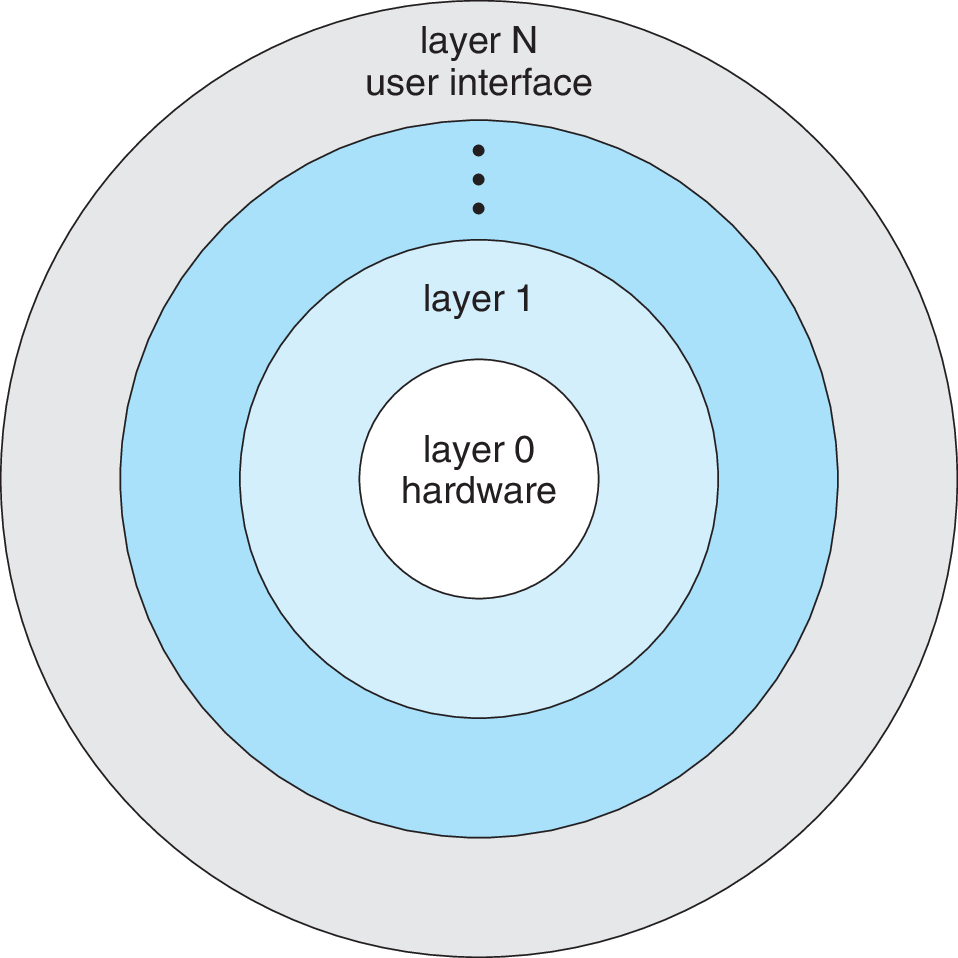
\includegraphics[width=4cm]{figs/00-2_13.pdf}
  \end{center}

\end{frame}

%---------------------------------------------------------------------
\begin{frame}
  \frametitle{Estructura: {\em microkernels}}

  {\bf Mach}: versión de UNIX usando diseño de {\em microkernel} (CMU)
  
  \begin{itemize}
    \item Set de funcionalidades mínimas
    \item Otras funcionalidades agregadas como programas de usuario ¿dónde poner el límite?
    \item<2-> {\bf Darwin} (MacOS X kernel) basado parcialmente en modelo Mach
    \item<3-> Ventaja: Sistemas pequeño y fácil de portar
    \item<4-> Desventaja: Más interacción a través de {\em syscalls}
    \item<4-> {\bf Windows NT} usaba microkernel pero era más lento que Win95.
  \end{itemize}

  \begin{center}
    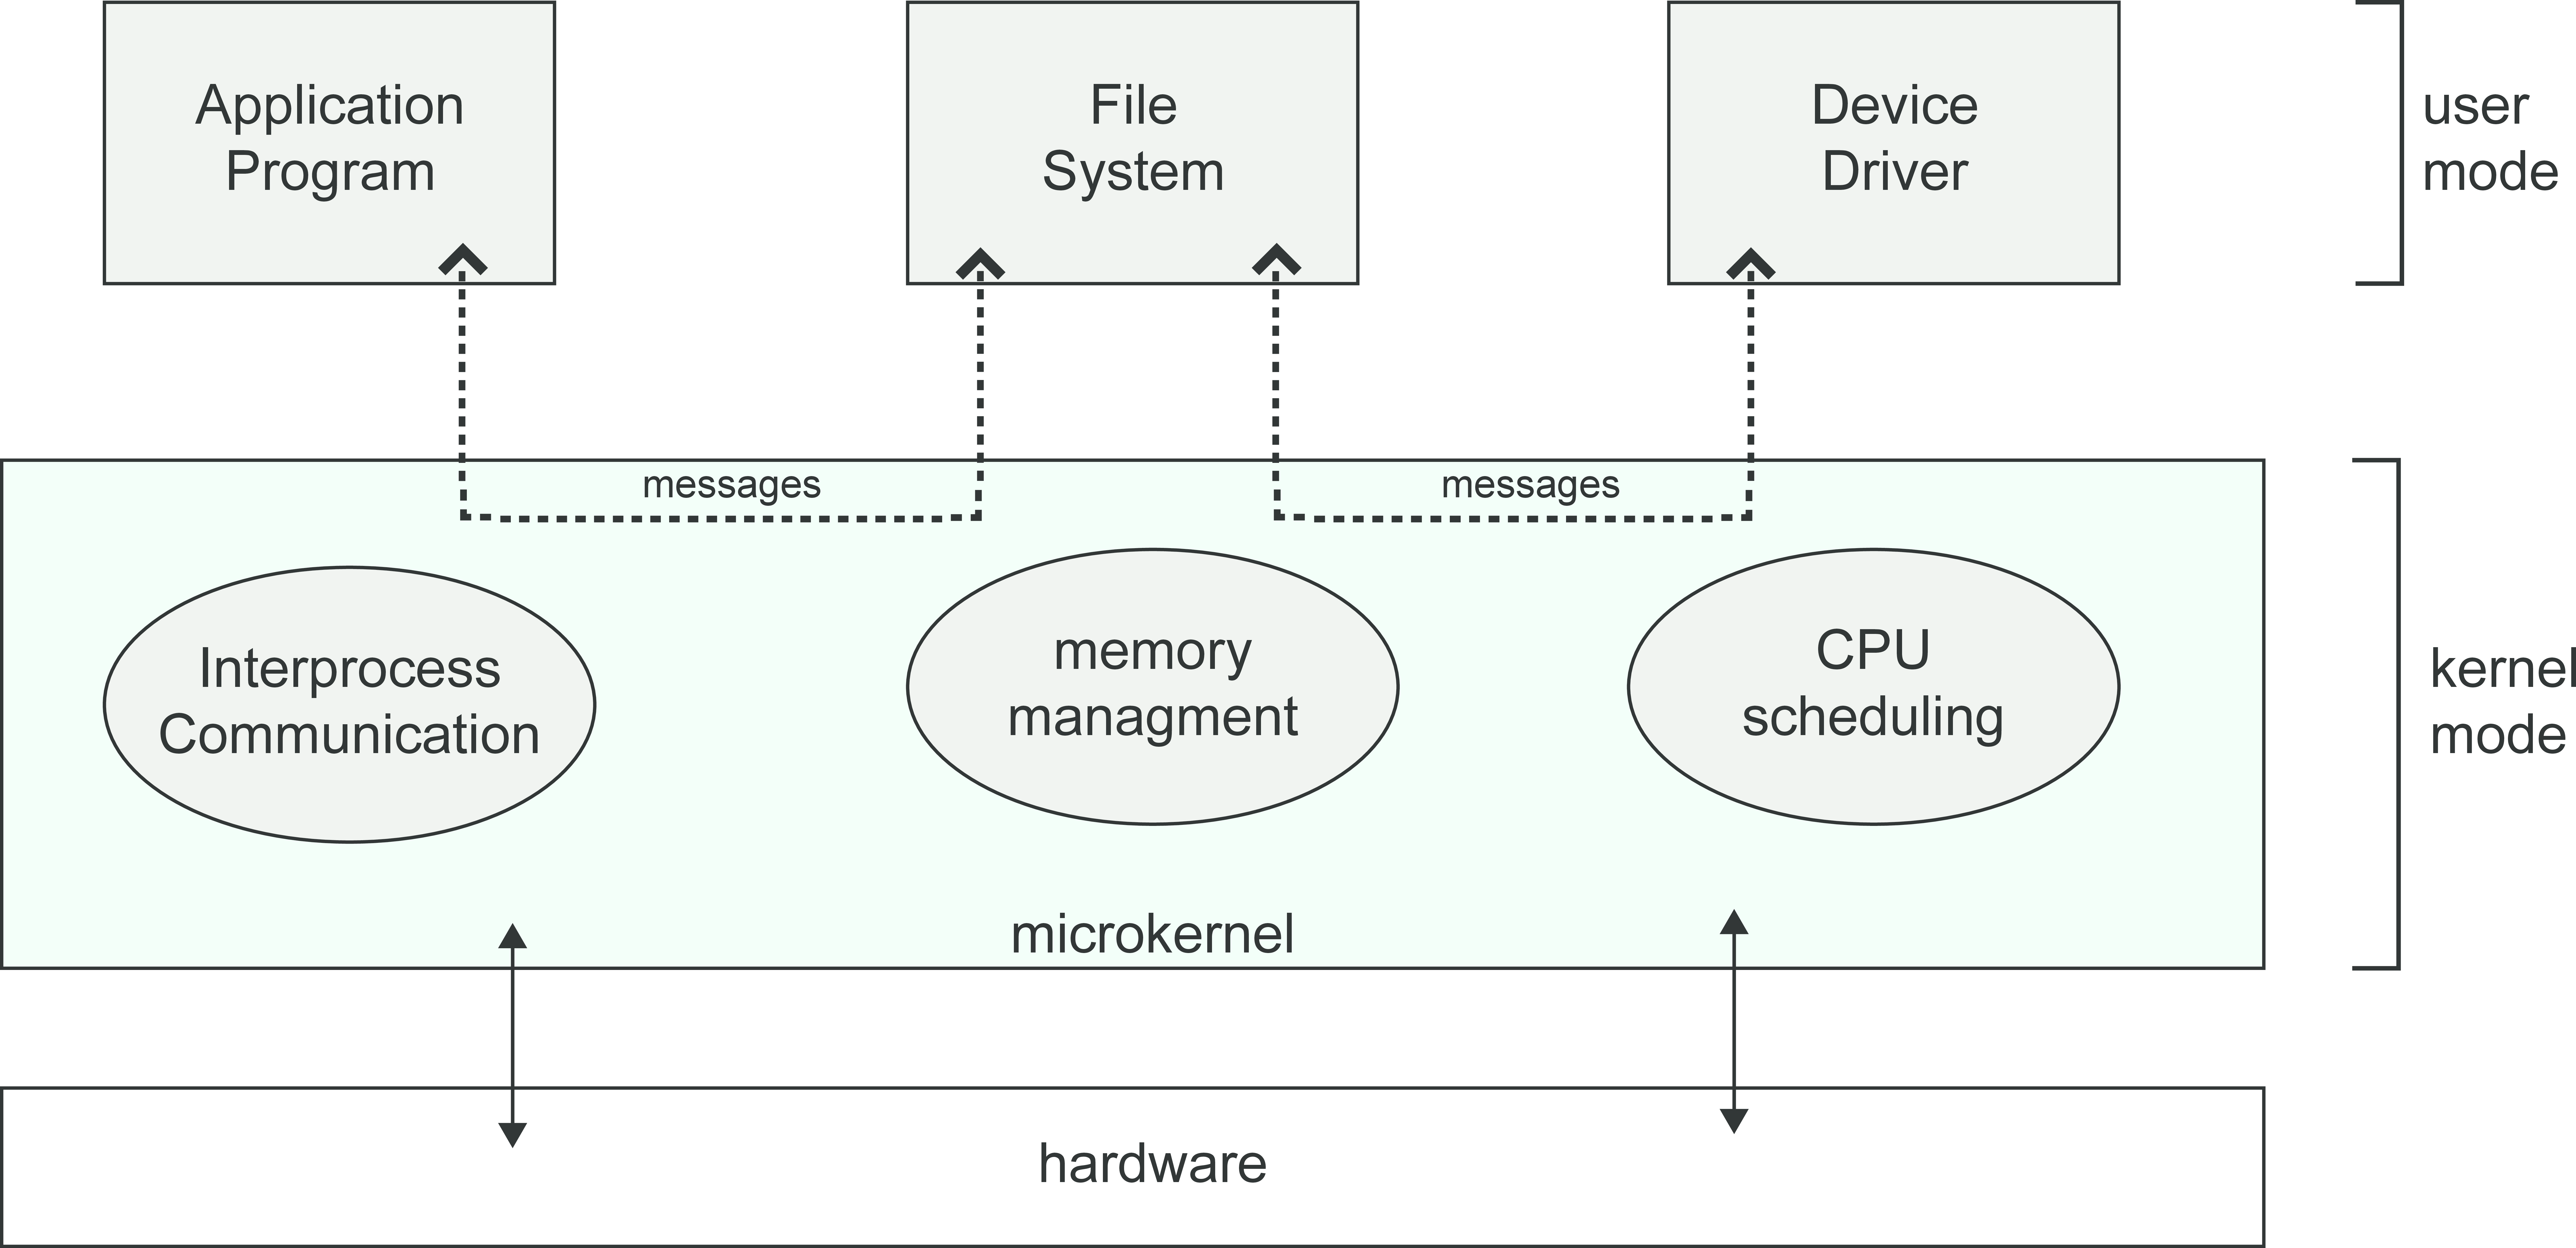
\includegraphics[width=6cm]{figs/00-2_14.pdf}
  \end{center}

\end{frame}

%---------------------------------------------------------------------
\begin{frame}
  \frametitle{Estructura: {\em módulos}}

  Lo más común: {\bf loadable kernel modules}
  \begin{itemize}
    \item Kernel tiene un conjunto de componentes principales ({\em core})
    \item Módulos necesarios se agregan durante ejecución
    \item Evita recompilar el kernel para cada nueva funcionalidad
    \item Solaris, Linux, MacOS X, Windows
    \item Ej: kernel con soporte de manejo de archivo + módulos por cada {\em filesystem}
  \end{itemize}

  \begin{center}
    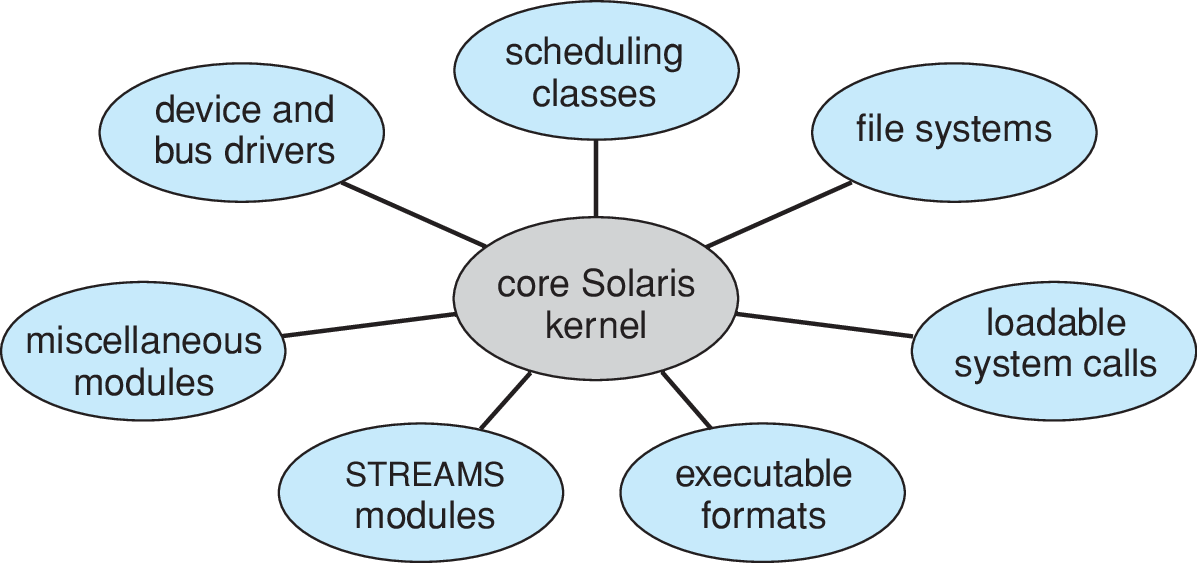
\includegraphics[width=6cm]{figs/00-2_15.pdf}
  \end{center}


\end{frame}

%---------------------------------------------------------------------
\begin{frame}
  \frametitle{Al final: Estructuras híbridas}

  En la práctica, pocos sistemas pueden ser encasillados
  \begin{itemize}
    \item Linux, Solaris, Windows tienen características monolíticas (performance!)
    \item Pero algunas funcionalidades siguen el diseño de {\em microkernel}
    \item ¡Y además permiten cargar módulos dinámicamente!
  \end{itemize}

\end{frame}

%---------------------------------------------------------------------
%\begin{frame}
%  \frametitle{Ejemplo: Apple Mac OS X}
%
%  \begin{itemize}
%    \item {\bf Cocoa}: API para Objective-C
%    \item Kernel: Mach microkernel + BSD Unix Kernel
%      \begin{itemize}
%        \item Mach: manejo de memoria, RPC, IPC, paso de mensajes, {\em threads}
%        \item BSD: CLI, networking, sistemas de archivos, API POSIX
%      \end{itemize}
%    \item Módulos cargables: {\bf kernel extensions}
%  \end{itemize}
%  
%  \begin{center}
%    \includegraphics[width=7cm]{figs/00-2_16.pdf}
%  \end{center}
%
%\end{frame}

%---------------------------------------------------------------------
%\begin{frame}
%  \frametitle{Ejemplo: Apple iOS}
%
%  \begin{itemize}
%    \item {\bf Cocoa Touch} = Cocoa + soporte para gestos
%    \item Media: soporte gráfico + audio + video
%    \item Core: kernel basado en Mac OS X
%  \end{itemize}
%
%  \begin{center}
%    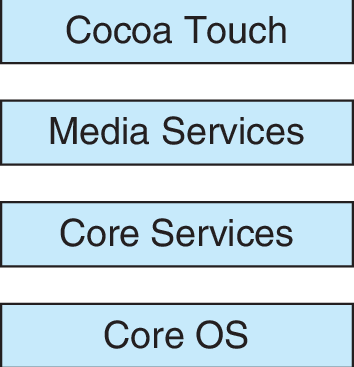
\includegraphics[width=4cm]{figs/00-2_17.pdf}
%  \end{center}
%
%\end{frame}

%---------------------------------------------------------------------
%\begin{frame}
%  \frametitle{Ejemplo: Android}
%
%  \begin{itemize}
%    \item Modelo por capas + kernel Linux
%    \item Implementación de máquina virtual {\bf Dalvik}
%    \item Frameworks para desarrollo: webkit, SQLite, libc
%  \end{itemize}
%
%  \begin{center}
%    \includegraphics[width=6cm]{figs/00-2_18.pdf}
%  \end{center}
% 
%\end{frame}


\end{document}